\documentclass[10pt]{article}

\usepackage[letterpaper,left=1.5in,right=1.5in,top=1in,bottom=1in]{geometry}
\usepackage{newtxtext,newtxmath}
\usepackage{graphicx}
\usepackage{booktabs}
\usepackage{amsmath}
\usepackage{caption}
\usepackage{titlesec}
\usepackage[hidelinks]{hyperref}

\Urlmuskip=0mu plus 1mu\relax
\def\UrlBreaks{\do\/\do-\do.\do\_}

\graphicspath{{../figures/}}
\captionsetup{font=small,labelfont=bf}
\titleformat{\section}{\normalfont\large\bfseries}{\thesection}{0.7em}{}
\titleformat{\subsection}{\normalfont\normalsize\bfseries}{\thesubsection}{0.6em}{}
\titlespacing*{\section}{0pt}{1.1em}{0.4em}
\titlespacing*{\subsection}{0pt}{0.8em}{0.3em}

\hypersetup{
  pdftitle={Predicting stock prices with LSTM Networks},
  pdfauthor={David Duemig},
}

\input{generated/macros}

\begin{document}

\begin{center}
  {\noindent\rule{\textwidth}{1.2pt}}\\[0.7em]
  {\LARGE\bfseries Predicting stock prices with LSTM Networks}\\[0.5em]
  {\noindent\rule{\textwidth}{1.2pt}}\\[1.0em]
  {\large David Duemig}\\[1.2em]
\end{center}

\begin{abstract}
We ask whether a long short term memory (LSTM) network can predict the direction
of the S\&P 500 over the next month from past returns, volatility and trading
volume, and whether it does so any better than a regularised logistic
regression. We use one non-overlapping observation per month, build stationary
features, and validate with purged walk-forward cross-validation so that no
future information leaks into the past. On a held-out test set of \nTest{} months
the LSTM, the linear baseline and a gradient-boosting model all score close to
the naive rule of always predicting ``up''. Test AUCs lie between \minAUC{} and
\maxAUC{}, and no model beats the base rate by a margin that survives a
block-bootstrap confidence interval. A probability threshold trained only on
validation data does not produce a timing strategy that beats buying and holding
after costs. Monthly index direction remains very hard to predict from price and
volume alone.
\end{abstract}

\section{Introduction}

Artificial intelligence now performs many tasks that once needed an expert. In
finance this has encouraged a search for models that forecast asset returns.
Models of individual stock returns usually start from company and market
characteristics, and most studies form their predictions with simple linear
models \cite{blitz,lewellen}. A growing literature argues that machine learning
and deep learning, which allow nonlinear interactions between predictors, can
improve these forecasts \cite{freyberger,gu,rapach}.

This project asks a narrow version of that question. We train LSTM networks on
time-series price and volume data for the S\&P 500 and compare their
out-of-sample predictability with that of a regularised logistic regression and
a gradient-boosting classifier. The task is a monthly up or down call on the
index. The headline result is negative, and we report it as it comes out: the
problem is close to unpredictable at this horizon from these inputs.

\section{Related work}

Successful financial models are usually proprietary, so published work with
state-of-the-art performance on this exact task is scarce. The academic
community has nonetheless taken up deep learning in finance, and the LSTM is a
common choice for sequence data. Gao applied an LSTM to forecast six US
industries from 359 features \cite{gao}. Nelson et al predicted short-horizon
direction from technical features \cite{nelson}, and Chen et al used an LSTM on
historical prices to classify daily moves \cite{chen}. Lopez de Prado documents
why ordinary cross-validation leaks in finance and proposes purging and an
embargo, which we adopt \cite{deprado}. Our features are standard momentum,
volatility and liquidity signals.

\section{Dataset and Features}

\subsection{Raw Data}

The data are daily quotes for the S\&P 500 price index (Yahoo ticker
\texttt{\^{}GSPC}) from \dataStart{} to \dataEnd{}, downloaded with
\texttt{yfinance}. Each row has the open, high, low, close and volume. We use the
close and the volume. The raw series has about \nRawRows{} trading days.
Re-downloading later may give marginally different values, which does not change
the conclusions.

\subsection{Features}

All features are stationary, which matters because the model must generalise
across four decades in which the index level and the traded volume both grew by
large factors. From the daily close we form log returns,
\begin{equation}
  r_t = \ln\!\left(\frac{P_t}{P_{t-1}}\right).
\end{equation}
For each look-back window of $w$ weeks (five trading days per week), with $w$ in
$\{1,2,3,4,8,12,\dots,80\}$, we compute three month-end features: the summed log
return over the window, the standard deviation of daily returns over the window,
and a detrended log volume. The first two are stationary by construction. For
volume we subtract a trailing one-year mean of log volume from the window mean of
log volume,
\begin{equation}
  \text{volume}_{w,t} = \overline{\ln V}_{\,t,\,5w} - \overline{\ln V}_{\,t,\,252},
\end{equation}
which removes the strong secular growth in turnover. This gives 23 windows for
each of the three families and \nFeatures{} month-end features in total. The
three families, volatility, return and volume, are combined into the seven models
of the original project (each family alone, each pair, and all three).

The LSTM does not see these aggregates. It receives the most recent \lookback{}
trading days of the daily channels that correspond to the chosen families: the
daily log return, a rolling daily volatility, and the detrended daily log volume.
This lets the network read a real sequence rather than a single snapshot.

\subsection{Scaling}

Features are rescaled before training so that the optimiser sees comparable
magnitudes and the penalty treats coefficients evenly. We use standardisation,
which centres each feature and scales it to unit variance,
\begin{equation}
  X^{(i)}_z = \frac{X^{(i)} - \bar X}{s_X}.
\end{equation}
The scaler is fitted inside each cross-validation fold on the training part only,
never on the validation or test months, so no scaling information leaks forward.
The LSTM channels are standardised the same way, using statistics from the
training sequences only.

\subsection{Separating Test Data}

Ordinary k-fold cross-validation fails in finance because it mixes future and
past \cite{deprado}. We instead hold out the last \testFrac{} of the months as a
test set, used once after everything is fixed, and tune on the earlier months
with walk-forward cross-validation. Because each label looks one month ahead, a
training month whose label window reaches a validation month is purged, and a
further embargo of \embargo{} month is dropped before each validation block.
Figure~\ref{fig:walkforward} shows the scheme.

\begin{figure}[t]
  \centering
  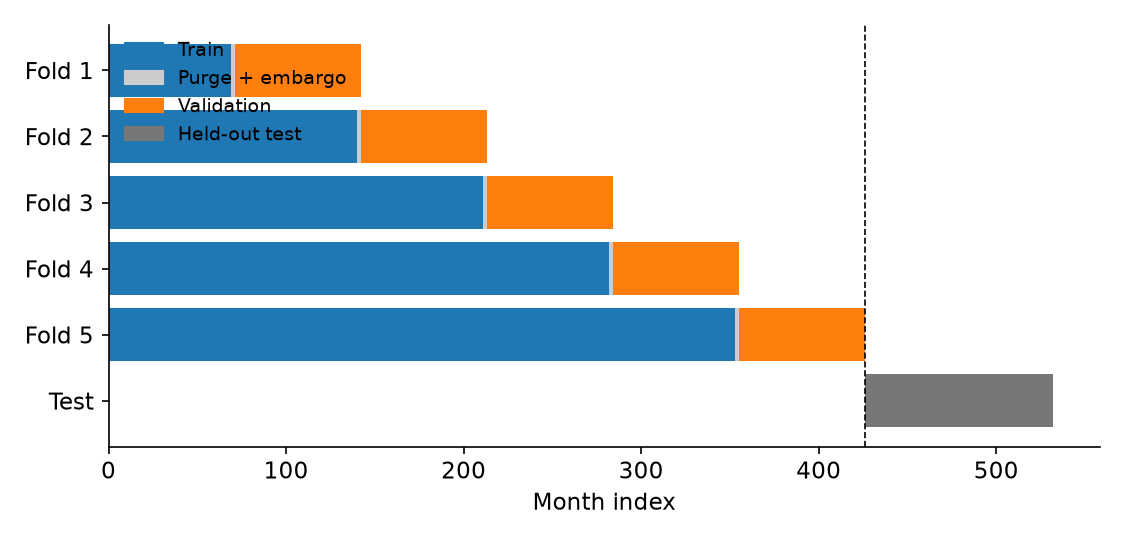
\includegraphics[width=0.92\textwidth]{walk_forward.png}
  \caption{Purged walk-forward cross-validation on the development months. Each
  fold trains on an expanding block of past months, skips a purge and embargo
  gap, and validates on the next block. The final months are held out as the
  test set.}
  \label{fig:walkforward}
\end{figure}

\subsection{Label Distribution}

Each month is labelled up or down by the sign of the next month's return. Using
one non-overlapping observation per month removes the heavy overlap of the
original daily labelling, at the cost of a small sample: \nMonths{} months after
the feature warm-up, of which \nDev{} are development months and \nTest{} are test
months. The classes are unbalanced in favour of ``up'': \devUp{} of development
months and \testUp{} of test months are up. This imbalance is central to reading
the results, because a model that always predicts ``up'' already scores
\testUp{} on the test set.

\section{Models}

\subsection{Baseline Models}

Two baselines use the month-end aggregates. The first is a logistic regression
with an elastic-net penalty, which spans ridge and lasso, trained with the saga
solver. The penalty strength and the L1 ratio are tuned by the walk-forward
cross-validation above. The second is a gradient-boosting classifier, tuned over
its learning rate and tree size on the same folds. We also report the naive
always-up rule, which is the benchmark every model has to beat.

\subsection{LSTM Networks}

The LSTM reads a sequence of \lookback{} trading days and outputs the probability
of an up month through a single sigmoid unit (Figure~\ref{fig:network}). An LSTM
keeps a cell state across time steps and uses forget, input and output gates to
decide what to keep, add and read out, which lets it learn longer dependencies
than a plain recurrent network \cite{colah}. Because the sample is small, the
architecture is kept deliberately small and is not tuned; instead we train it
with early stopping and average over \nSeeds{} random seeds, reporting the mean
and the spread.

\begin{figure}[t]
  \centering
  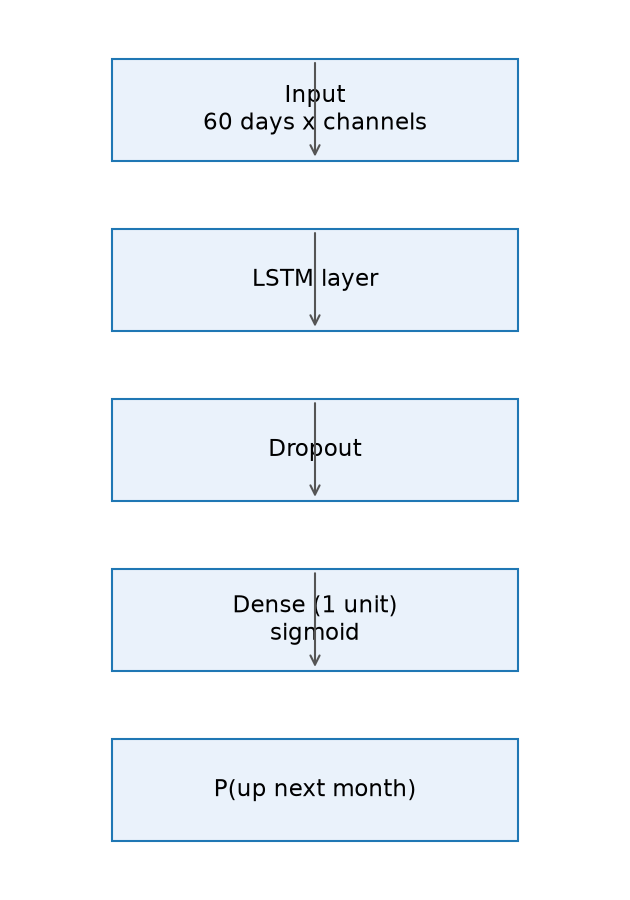
\includegraphics[width=0.42\textwidth]{network_structure.png}
  \caption{Network structure. A sequence of daily feature channels feeds one LSTM
  layer, a dropout layer and a single sigmoid output.}
  \label{fig:network}
\end{figure}

\subsection{Experiment Design}

For each of the seven feature sets we fit the elastic-net baseline, the
gradient-boosting baseline and the LSTM. We score each model on the test months
by accuracy, by the area under the ROC curve (AUC) and by the Brier score, and we
attach 95\% confidence intervals from a moving-block bootstrap over months, which
preserves any serial dependence. We also compare each model with the always-up
rule month by month and report whether the difference is positive after the
bootstrap. Finally we test a simple timing strategy: hold the index next month
when the predicted probability of an up month exceeds a threshold chosen on
validation data only, otherwise hold cash, and charge a transaction cost of
\cost{} on each change in position.

\subsection{Experiment Results}

Table~\ref{tab:classification} summarises the classification results and
Figure~\ref{fig:auc} plots the test AUCs with their intervals. The picture is
consistent across models and feature sets. Test AUCs cluster around 0.5, from
\minAUC{} to \maxAUC{}, and all but one of the intervals contain 0.5. The best
test accuracy is \maxAcc{}, equal to the always-up rate of \testUp{}; no model
beats always-up by an accuracy margin whose confidence interval excludes zero. One
of the twenty-one model and feature-set combinations, the elastic net on all three
families, has an AUC interval that just clears 0.5. With twenty-one combinations
this is close to what chance alone produces, and that same model's accuracy does
not beat always-up.

\begin{table}[t]
  \centering
  \caption{Test-set accuracy and AUC for each model and feature set, with the
  always-up benchmark. EN is the elastic-net logistic regression and GB the
  gradient-boosting model. The test set has \nTest{} months with an up rate of
  \testUp{}.}
  \label{tab:classification}
  \input{generated/table_classification}
\end{table}

\begin{figure}[t]
  \centering
  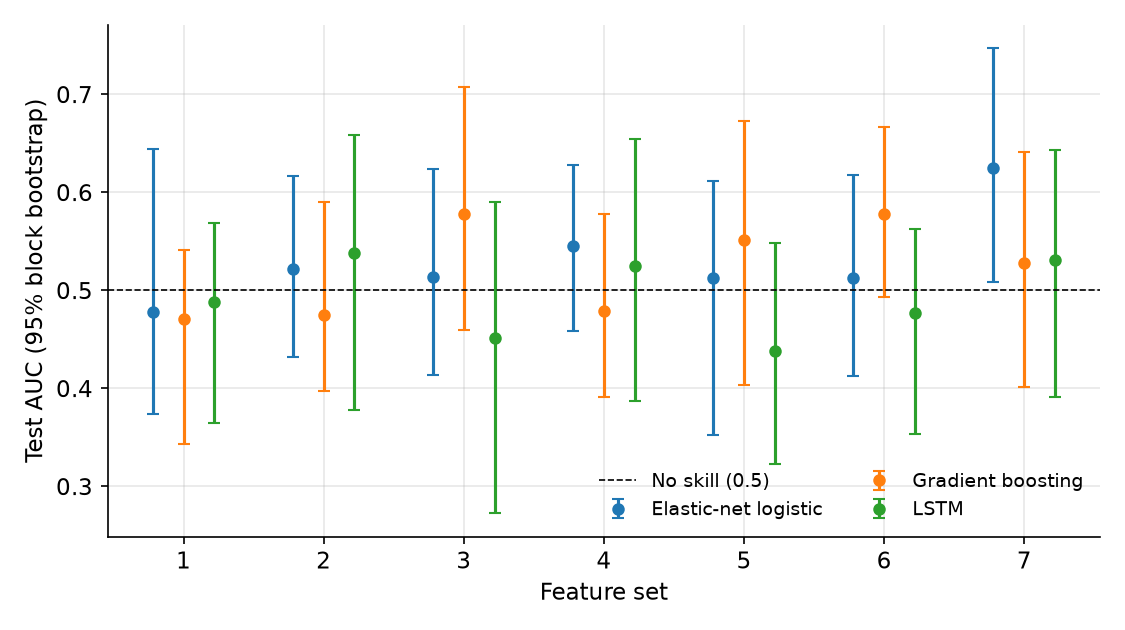
\includegraphics[width=0.92\textwidth]{auc_by_model.png}
  \caption{Test AUC by feature set and model, with 95\% block-bootstrap
  intervals. The dashed line marks 0.5, the no-skill level.}
  \label{fig:auc}
\end{figure}

The economic test tells the same story. Table~\ref{tab:strategy} and
Figure~\ref{fig:equity} compare buying and holding with the best timing strategy
per model family. Buy-and-hold earns an annual return of \bhReturn{} at a Sharpe
ratio of \bhSharpe{} over the test period. The best timing strategy reaches a
Sharpe of \bestSharpe{}, but it is the best of twenty-one model and feature-set
combinations, and most strategies simply stay invested and recover buy-and-hold.
An edge of this size is well within what picking the best of many would produce,
so it is not evidence of genuine timing skill.

\begin{table}[t]
  \centering
  \caption{Annualised test performance, buy-and-hold against the best timing
  strategy per model family, after costs.}
  \label{tab:strategy}
  \input{generated/table_strategy}
\end{table}

\begin{figure}[t]
  \centering
  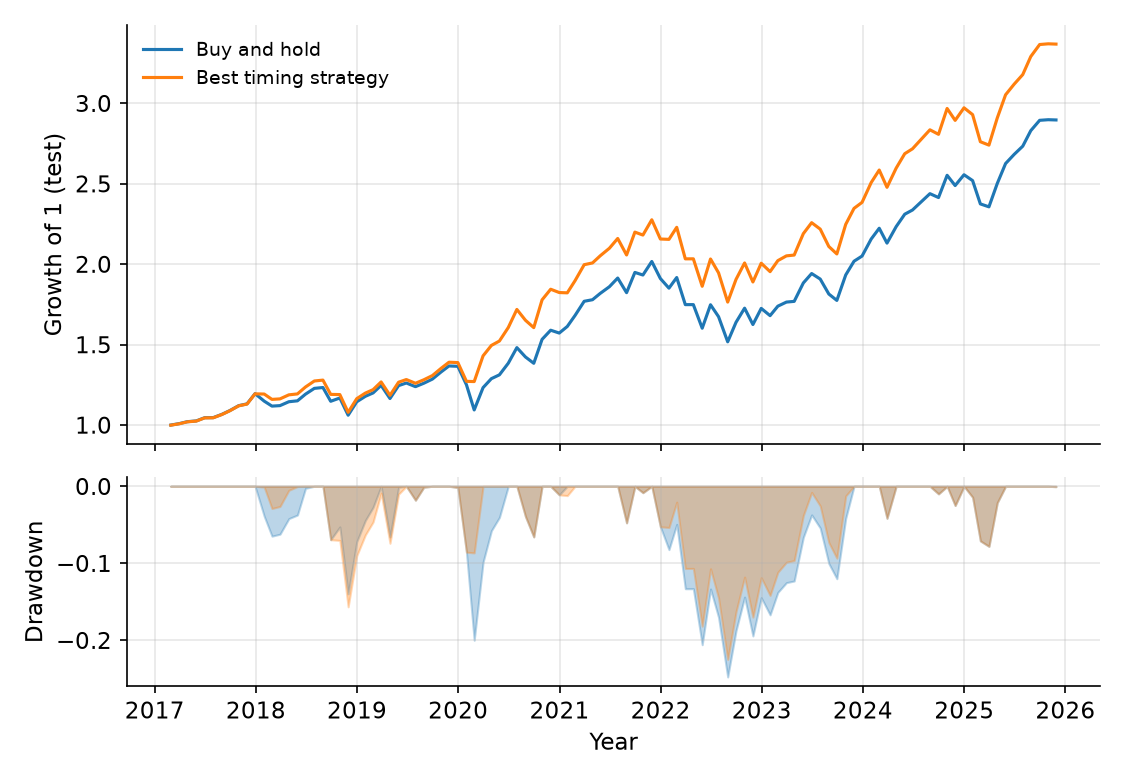
\includegraphics[width=0.92\textwidth]{strategy_equity.png}
  \caption{Growth of one unit over the test period for buy-and-hold and the best
  timing strategy, with drawdowns below.}
  \label{fig:equity}
\end{figure}

\section{Conclusion and Future Work}

Monthly index direction remains very hard to predict even after cleaning up the
method. With non-overlapping labels, purged validation, stationary features and a
sequence model that sees real history, the LSTM, the linear baseline and the
gradient-boosting model all sit close to the always-up rule, and the timing
strategy does not beat buying and holding after costs. One honest reading is that
price and volume do not carry enough information about the next month's direction,
and that the strong upward drift of the index makes the base rate hard to beat.
Useful next steps are to add information beyond price and volume, such as
fundamentals or macro data; to predict a continuous return or a quantile rather
than a sign; and to study a longer or international sample so that the test set is
not dominated by a single bull market.

\section*{Acknowledgements}

This project began as a course project for CS230 Deep Learning. I thank the
teaching team and my advisor Sagar Honnungar.

\begin{thebibliography}{10}
\small
\bibitem{blitz} Blitz, D. \& Vidojevic, M. (2018), `The Characteristics of Factor Investing', SSRN Electronic Journal, \url{https://ssrn.com/abstract=3206798}.
\bibitem{lewellen} Lewellen, J. (2015), `The Cross-section of Expected Stock Returns', Critical Finance Review, vol.~4, no.~1, pp.~1--44, \url{https://ssrn.com/abstract=2511246}.
\bibitem{freyberger} Freyberger, J., Neuhierl, A. \& Weber, M. (2017), `Dissecting characteristics nonparametrically', CESifo Working Paper 6391, \url{https://ssrn.com/abstract=2935432}.
\bibitem{gu} Gu, S., Kelly, B.T. \& Xiu, D. (2018), `Empirical Asset Pricing via Machine Learning', Chicago Booth Research Paper 18-04, \url{https://ssrn.com/abstract=3159577}.
\bibitem{rapach} Rapach, D., Strauss, J., Tu, J. \& Zhou, G. (2018), `Industry Return Predictability: A Machine Learning Approach', SSRN Electronic Journal, \url{https://ssrn.com/abstract=3120110}.
\bibitem{gao} Gao, Q. (2016), `Stock market forecasting using recurrent neural network', University of Missouri, Columbia.
\bibitem{chen} Chen, K., Zhou, Y. \& Dai, F. (2015), `A LSTM-based method for stock returns prediction', Proceedings of the 2015 IEEE International Conference on Big Data, pp.~2823--2824.
\bibitem{nelson} Nelson, D.M., Pereira, A.C. \& de Oliveira, R.A. (2017), `Stock markets movement prediction with LSTM neural networks', Proceedings of the 2017 International Joint Conference on Neural Networks, pp.~1419--1426.
\bibitem{deprado} Lopez de Prado, M. (2018), `Advances in Financial Machine Learning', Wiley, New Jersey.
\bibitem{colah} Olah, C. (2015), `Understanding LSTM Networks', \url{http://colah.github.io/posts/2015-08-Understanding-LSTMs/}.
\end{thebibliography}

\section*{Github Repository}

{\small\sloppy\url{https://github.com/duemig/Stanford-Project-Predicting-stock-prices-using-a-LSTM-Network}\par}

\end{document}
